\section{Simuleringsvindu}
\thispagestyle{fancy}

Når ein testar og simulerer eit program kan det bli mange variablar og komponentar
å halde styr på. Derfor er det viktig å sorterer og behalde relevant informasjon, 
samt å kunne presentere den på ein god måte.

\gls{Codesys} Visualization\citep{CodesysVizualisation} er eit grafisk verktøy der ein kan presentere informasjon
ved hjelp av grafiske element. Dette gav oss moglegheit til å presentere tankar, ventilar og pumper
ved hjelp av bilete og lys. 
Dette gjorde det mykje lettare for oss og oppdage eventuelle feil eller fastslå at ting fungerte som dei skulle.

Vi brukte visualiseringsverktøyet til å lage eit fullskala simuleringsvindu, der kvar komponent
vart knytt til sitt spesifikke grafiske symbol. Dette vindauget brukte vi saman med simuleringa
av programmet og knytte dei relevante inngangssignala til knappar. 
Dette gjorde at vi til slutt hadde eit grensesnitt mot programmet og kunne enkelt simulere
forskjellige driftssituasjonar og konkludere med eit resultat.

Simuleringsvindauget er ikkje noko \gls{HMI} og tar ikkje omsyn til aktuelle normer og krav.

\begin{figure}[htbp]
    \centering
    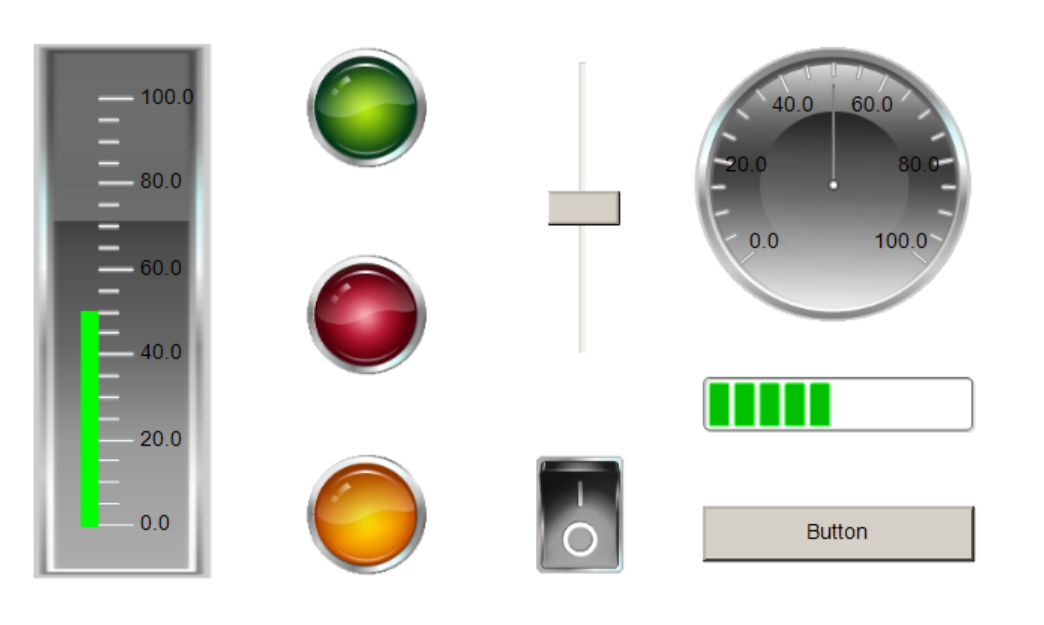
\includegraphics[width=0.8\textwidth]{Bilder/Codesys symbol.png}
    \caption{Eksempel \gls{Codesys} visualisering}\label{fig:CodesysVisualisering}
\end{figure}

\newpage
